\documentclass{article}
\usepackage[utf8]{inputenc}
\usepackage{url}
\usepackage{amsmath,amsthm,enumitem}
\usepackage{graphicx}
\usepackage{lscape}
\usepackage{geometry}
\usepackage{color}
\usepackage{float}
\usepackage{listings}
\usepackage{amssymb}
\usepackage{verbatim}
\usepackage{algpseudocode} 
\usepackage{algorithm}
\usepackage{algorithmicx}  
\usepackage{hyperref}
\usepackage{courier}
\usepackage{listings} 
\usepackage{subcaption}
\usepackage{algorithm,algpseudocode}
\DeclareMathOperator*{\argmax}{arg\,max}
\DeclareMathOperator*{\argmin}{arg\,min}
\geometry{left=2.5cm,right=2.5cm,top=2.5cm,bottom=2.5cm} 
\renewcommand{\baselinestretch}{2}
\setcounter{MaxMatrixCols}{20}
\algnewcommand{\Inputs}[1]{%
  \State \textbf{Inputs:}
  \Statex \hspace*{\algorithmicindent}\parbox[t]{.8\linewidth}{\raggedright #1}
}
\algnewcommand{\Initialize}[1]{%
  \State \textbf{Initialize:}
  \Statex \hspace*{\algorithmicindent}\parbox[t]{.8\linewidth}{\raggedright #1}
}

\theoremstyle{definition}
\newtheorem{definition}{Definition}

\theoremstyle{plain}
\newtheorem{theorem}{Theorem}
\newtheorem{lemma}{Lemma}
\newtheorem{remark}{Remark}
\newcounter{example}[section]
\newenvironment{example}[1][]{\refstepcounter{example}\par\medskip
   \noindent \textbf{Example~\theexample. #1} \rmfamily}{\medskip}

\title{Note on Matching}
\author{Haocheng Dai}
\date{\today}
\DeclareUnicodeCharacter{2212}{-}
\begin{document}
\maketitle

\section{Metric}
\subsection{Information metric}
In information geometry, the Fisher information metric is a particular Riemannian metric which can be defined on a smooth statistical manifold, i.e., a smooth manifold whose points are probability measures defined on a common probability space. It can be used to calculate the informational difference between measurements.

\section{Density Matching}
\subsection{Sobolev $\Dot H^1$ metric and Fisher-Rao metric}
The right-invariant Sobolev $\Dot H^1$ metric on the quotient space Dens($M$) of probability densities on $M$ coincides with the Fisher-Rao metric on any $k$-dimensional statistical submanifold of Dens($M$)(Theorem 4.4 in \cite{khesin}).

\begin{definition}
The Fisher-Rao metric is the Riemannian metric on $\mathrm{Dens(M)}$ given by
\begin{equation*}
    G_\rho(\Dot\rho,\Dot\rho)=\frac{1}{4}\int_M\frac{\Dot{\rho}^2}{\rho}dx
\end{equation*}
\end{definition}

\begin{remark}
Given $\rho_0,\rho_1\in\mathrm{Dens(M)}$ with the same total mass, the Riemannian distance w.r.t. the Fisher-Rao metric is given by
\begin{equation*}
    \mathrm{dist}^2_{FR}(\rho_0,\rho_1)=\arccos\left(\int_M\sqrt{\frac{\rho_1}{\rho_0}}\rho_0\right)
\end{equation*}
$\rho(t)$ is the unique Fisher-Rao geodesic connecting $\rho_0$ and $\rho$, which can be calculated as
\begin{equation*}
    \rho(t)=\left(\frac{\sin((1-t)\theta)}{\sin(\theta)}+\frac{\sin(t\theta)}{\sin(\theta)}\sqrt{\frac{\rho}{\rho_0}}\right)^2\rho_0
\end{equation*}
where $\theta$ is the Riemannian distance w.r.t the Fisher-Rao metric
\begin{equation*}
    \theta=\mathrm{dist}_{FR}(\rho,\rho_0)=\arccos\int_M\sqrt{\frac{\rho}{\rho_0}}\rho_0
\end{equation*}
\end{remark}

\begin{remark}
The Fisher-Rao metric is the unique Riemannian metric on the space of probability densities that is invariant under the action of the diffeomorphism group
\begin{align*}
    \mathrm{dist}^2_{FR}(I_0dx,I_1dx)=d^2_{FR}(\phi_*(I_0dx),\phi_*(I_1dx)) &&\forall \phi\in \mathrm{Diff}(\Omega)
\end{align*}
\end{remark}

\begin{remark}
As the figure below shows, Hellinger distance $\mathrm{dist}_{Hel}(\lambda, \nu)$ is extrinsic, while the spherical Hellinger distance is intrinsic, which denoted as $\mathrm{dist}_{\Dot{H}^1}(\lambda, \nu)$. When seeing from a microscopic view, $\mathrm{dist}_{Hel}(\lambda, \nu)$ and $\mathrm{dist}_{\Dot{H}^1}(\lambda, \nu)$ can be regarded as the same.
\begin{figure}[H]
\centering
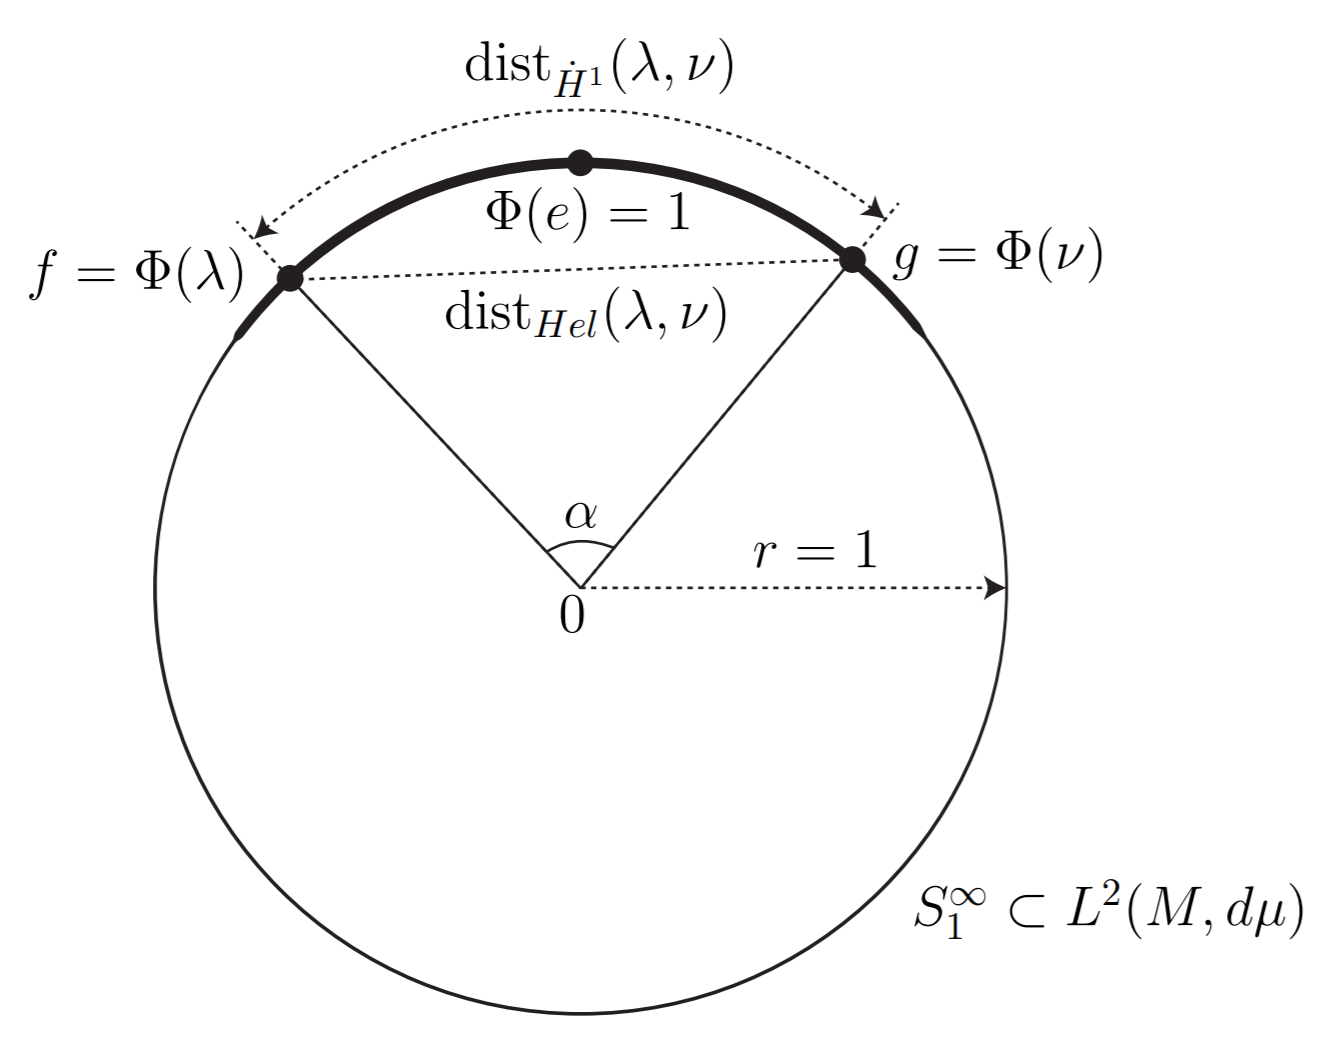
\includegraphics[scale=0.3]{figure/hellinger.png}
\caption{Hellinger distance and $\Dot H^1$ distance(spherical Hellinger distance)}
\end{figure}
\end{remark}

\begin{remark}\label{remark:fr}
Fisher-Rao distance and Hellinger distance are different, which are intrinsic and extrinsic, respectively, but they are magically equivalent. So we are using Hellinger distance to calculate energy in 2.2.
\end{remark}

\subsection{Exact density matching}
Given a probability distribution $I\in\mathrm{Prob}(M)$, find a diffeomorphism $\phi\in\mathrm{Diff}(M)$ that minimizes the energy function
\begin{align*}
    E(\phi)=\mathrm{dist}^2_{G^I}(\mathrm{id},\phi)\\
    \text{subject to }\phi_*I_0=I
\end{align*}
where $\phi_*$ is the push-forward of $\phi$ acting on densities $\phi_*I_0=|D\phi^{-1}|I_0\circ\phi^{-1}$, $G^I$ is the information metric, as shown below
\begin{align*}
    G^I_\phi(U,V)=-\int_M\langle\Delta u,v\rangle_g \mathrm{vol}+\lambda\sum^k_{i=1}\left(\int_M\langle u,\xi_i\rangle_g \mathrm{vol}\cdot\int_M\langle v,\xi_i\rangle_g \mathrm{vol}\right)\\
    G^I_\mathrm{id}(u,v)=-\int_M\langle\Delta u,v\rangle_g \mathrm{vol}+\lambda\sum^k_{i=1}\left(\int_M\langle u,\xi_i\rangle_g \mathrm{vol}\cdot\int_M\langle v,\xi_i\rangle_g \mathrm{vol}\right)
\end{align*}
where $U=u\circ\phi, V=v\circ\phi, \lambda>0, \Delta$ is the Laplace-de Rham operator lifted to vector fields, and $\xi_1,\cdots,\xi_k$ is an orthonormal basis of the harmonic 1-form on $M$.

The metric $G^I$ has the property of right-invariance: if $U,V\in T_\phi\mathrm{Diff}(M)$ then
\begin{align*}
    G^I_\phi(U,V)=G^I_{\phi\circ\psi}(U\circ\psi,V\circ\psi) && \forall\psi\in\mathrm{Diff}(M)
\end{align*}



\begin{algorithm}  
\caption{Optimal Information Transport}\label{algo1}
    \begin{algorithmic}
        \State $K=\mathbb{Z}^+$
        \State $\varepsilon=1/K$
        \State $\phi_0=\mathrm{id}$
        \For{$k=1:iternum$}
            \State $t=\frac{k}{K}$
            \State $\theta=\arccos\int_M\sqrt{\frac{\mu}{\mu_0}}\mu_0$ \Comment{Riemannian distance w.r.t the Fisher-Rao metric}
            \State $\mu(t)=\left(\frac{\sin((1-t)\theta)}{\sin(\theta)}+\frac{\sin(t\theta)}{\sin(\theta)}\sqrt{\frac{\mu}{\mu_0}}\right)^2\mu_0$ \Comment{Compute Fisher-Rao geodesic}
            \State $\Dot{\mu}(t)=\frac{d}{dt}\mu(t)$ \Comment{Compute velocity}
            \State $f_k=\Delta^{-1}(\frac{\Dot{\mu}(t)}{\mu(t)}\circ\phi_k)$ \Comment{Solve the Poisson equation}
            \State $v_k=\nabla f_k$ \Comment{Compute the gradient of vector field}
            \State $\psi_k=\mathrm{id}-\varepsilon v_k$ \Comment{Construct approximations $\psi_k$}
            \State $\phi_{k+1}=\phi_k\circ\psi_k$ \Comment{Update the diffeomorphism}
        \EndFor
        \State \Return{$\phi$}
    \end{algorithmic}  
\end{algorithm}  

\subsection{Inexact density matching}
Given $I_0,I_1\in\mathrm{Dens}(M)$, find a diffeomorphism $\phi\in\mathrm{Diff}(M)$ that minimizes the energy function
\begin{align*}
    E(\phi)&=\sigma\mathrm{dist}_{FR}^2(\phi_*f,f\circ\phi^{-1})+\Bar{\mathrm{dist}}_{FR}^2(\phi_*I_0,I_1)\\  
     &\triangleright\text{Hellinger distance(remark [\ref{remark:fr}]): }\mathrm{dist}_{FR}^2(I_0,I_1)=\int_\Omega(\sqrt{I_0}-\sqrt{I_1})^2dx\\
     &=\int_\Omega(\sqrt{\phi_*f}-\sqrt{f\circ\phi^{-1}})^2dx+\int_\Omega(\sqrt{\phi_*I_0}-\sqrt{I_1})^2dx\\
     &=\int_\Omega(\sqrt{|D\phi|f\circ\phi^{-1}}-\sqrt{f\circ\phi^{-1}})^2dx+\int_\Omega(\sqrt{|D\phi^{-1}|I_0\circ\phi^{-1}}-\sqrt{I_1})^2dx\\
     &=\int_\Omega(\sqrt{|D\phi|}-1)^2f\circ\phi^{-1}dx+\int_\Omega(\sqrt{|D\phi^{-1}|I_0\circ\phi^{-1}}-\sqrt{I_1})^2dx\\
     &=\int_\Omega(1-\sqrt{|D\phi|})^2fdy+\int_\Omega(\sqrt{I_0}-\sqrt{|D\phi|I_1\circ\phi})^2dy\\
     &\triangleright\text{change of variables: }x\rightarrow\phi(y),dx\rightarrow|D\phi|dy,|D\phi^{-1}|\rightarrow\frac{1}{|D\phi|},
\end{align*}
where the first term is a regularity measure and the second is the similarity measure. The parameter $\sigma$ is balancing the two criteria.

\subsection{How to calculate the gradient of the energy function}
\begin{equation}
    E(\phi)=\int_\Omega(1-\sqrt{|D\phi|})^2fdy+\int_\Omega(\sqrt{I_0}-\sqrt{|D\phi|I_1\circ\phi})^2dy\label{energy}
\end{equation}

Our approach to minimize the functional of Eq.(\ref{energy}) is to use a simple Euler integration of the discretization of the gradient flow
\begin{equation*}
    \Dot{\phi}=-\nabla^{G^I}E(\phi)
\end{equation*}

\begin{remark}
The relationship between the gradient w.r.t. information metric and $L^2$ metric is that
\begin{equation*}
    \left<\nabla^{G^I}E,v\right>_{H^1}=\left<-\Delta(\nabla^{G^I}E),v\right>_{L^2}
\end{equation*}
Therefore the information metric above can be written more specifically as 
\begin{equation*}
    G^I_\phi(U,V)=\int_\Omega\left<-\Delta u,v\right>_{L^2}dx,
\end{equation*}
where $u=\nabla^{G^I}E$ is the $G^I-$gradient.
\end{remark}

The $G^I-$gradient of Eq.(\ref{energy}) is given by
\begin{equation*}
    \nabla^{G^I}E=-\Delta^{-1}\left[-\nabla\left(\left(1-\sqrt{|D\phi^{-1}|}\right)f\circ\phi^{-1}\right)-\sqrt{|D\phi^{-1}|I_0\circ\phi^{-1}}\nabla\left(\sqrt{I_1}\right)+\nabla\left(\sqrt{|D\phi^{-1}|I_0\circ\phi^{-1}}\right)\sqrt{I_1}\right]
\end{equation*}
\begin{proof}
Let $\phi(s)$ be a family of diffeomorphisms parameterized by the real variable $s$, such that
\begin{align*}
    \frac{d}{ds}\bigg\rvert_{s=0}\phi(s)=v\circ\phi(0)=v\circ\phi&&\triangleright\text{see remark(\ref{remark:2})}
\end{align*}
denoting $\phi(0)$ with $\phi$.

The variation of the first term
\begin{align*}
    \frac{d}{ds}\bigg\rvert_{s=0}E_1(\phi)&=\frac{d}{ds}\bigg\rvert_{s=0}\left(\int_\Omega(1-\sqrt{|D\phi|})^2f(y)dy\right)\\
    &=\int_\Omega\frac{d}{ds}\bigg\rvert_{s=0}(1-\sqrt{|D\phi|})^2f(y)dy\\
    &=\int_\Omega2(1-\sqrt{|D\phi|})\frac{d}{ds}\bigg\rvert_{s=0}(1-\sqrt{|D\phi|})f(y)dy\\
    &=\int_\Omega2(1-\sqrt{|D\phi|})\left(-\frac{d}{ds}\bigg\rvert_{s=0}\sqrt{|D\phi|}\right)f(y)dy\\
    &=\int_\Omega2f(y)(\sqrt{|D\phi|}-1)\cdot\frac{1}{2}\left(\sqrt{|D\phi|}\mathrm{div}(v)\circ\phi(y)\right)dy \\ &\triangleright\frac{d}{ds}\bigg\rvert_{s=0}\sqrt{|D\phi_s|}=\frac{1}{2}\sqrt{|D\phi|}\mathrm{div}(v)\circ\phi\text{, see remark(\ref{remark:4})}\\
    &=\int_\Omega f(y)(\sqrt{|D\phi(y)|}-1)\sqrt{|D\phi(y)|}\mathrm{div}(v)\circ\phi(y)dy
\end{align*}

\begin{remark}\label{remark:4}\cite{hinkle}
Let $\phi_s$ be a family of irrotational diffeomorphisms indexed by the real variable $s$ and satisfying
\begin{equation*}
    \phi_0=\phi, \frac{d}{ds}\bigg\rvert_{s=0}\phi_s=u\circ\phi.
\end{equation*}

Then the pushforward of the vector field $u$ is defined as
\begin{equation*}
    TP(u\circ\phi)=\frac{d}{ds}\bigg\rvert_{s=0}P\phi_s.
\end{equation*}

A straightforward computation then yields
\begin{align*}
    TP(u\circ\phi)&=2\frac{d}{ds}\bigg\rvert_{s=0}\sqrt{|D\phi_s|}\\
    &=\frac{1}{\sqrt{|D\phi|}}\frac{d}{ds}\bigg\rvert_{s=0}|D\phi_s|\\
    &=\sqrt{|D\phi|}\mathrm{div}(u)\circ\phi\\
\end{align*}
\end{remark}

By substituting $y$ with $\phi^{-1}(x)$, $dy$ with $|D\phi^{-1}(x)|dx$ and $|D\phi(y)|=\frac{1}{|D\phi^{-1}(x)|}$ (see remark(\ref{remark:1})), we have
\begin{align*}
    \frac{d}{ds}\bigg\rvert_{s=0}E_1(\phi)&=\int_\Omega f(\phi^{-1}(x))\left(\frac{1}{\sqrt{|D\phi^{-1}(x)|}}-1\right)\frac{1}{\sqrt{|D\phi^{-1}(x)|}}\mathrm{div}(v)\circ x|D\phi^{-1}(x)|dx\\
    &=\int_\Omega f\circ\phi^{-1}(x)(1-\sqrt{|D\phi^{-1}(x)|})\mathrm{div}(v(x))dx\\
    &=\left< f\circ\phi^{-1}(1-\sqrt{|D\phi^{-1}|}),\mathrm{div}(v)\right>_{L^2(\mathbb{R}^3)}\\
    &=-\left<\nabla\left(f\circ\phi^{-1}(1-\sqrt{|D\phi^{-1}}\right),v\right>_{L^2(\mathbb{R}^3)}\\
    &\triangleright\text{adjoint of the divergence is the negative gradient}
\end{align*}

\begin{remark}\label{remark:1}
\begin{align*}
    \phi\circ\phi^{-1}(x)&=x\\
    \frac{d\left(\phi\circ\phi^{-1}(x)\right)}{dx}&=\frac{dx}{dx}\\
    |D\phi(\phi^{-1}(x))|\cdot|D\phi^{-1}(x)|&=1&&\triangleright\text{Chain rule}\\
    |D\phi(y)|\cdot|D\phi^{-1}(x)|&=1\\
    |D\phi(y)|&=\frac{1}{|D\phi^{-1}(x)|}\\
\end{align*}
\end{remark}

The derivative of the second term
\begin{align*}
    \frac{d}{ds}\bigg\rvert_{s=0}E_2(\phi)&=\frac{d}{ds}\bigg\rvert_{s=0}\int_\Omega(\sqrt{I_0}-\sqrt{|D\phi|I_1\circ\phi})^2dy\\
    &=\frac{d}{ds}\bigg\rvert_{s=0}\int_\Omega I_0(y)-2\sqrt{|D\phi(y)|I_0(y)I_1\circ\phi(y)}+|D\phi(y)|I_1\circ\phi(y)dy\\
    &=\frac{d}{ds}\bigg\rvert_{s=0}\int I_0(y)-2\sqrt{I_0(y)}\sqrt{I_1\circ\phi(y)}\sqrt{|D\phi(y)|}dy\\
    &\triangleright \text{constant conservation of mass}\\
    &=\frac{d}{ds}\bigg\rvert_{s=0}\int -2\sqrt{I_0(y)}\sqrt{I_1\circ\phi(y)}\sqrt{|D\phi(y)|}dy \\
    & \triangleright I_0(y) \text{ has nothing to do with } s\\
    &=-2\int\left[\left(\nabla\sqrt{I_1}^Tv\right)\circ\phi(y)\sqrt{I_0(y)}\sqrt{|D\phi(y)|}+\sqrt{I_0(y)I_1\circ\phi(y)}\frac{1}{2}\sqrt{|D\phi(y)|}\mathrm{div}(v)\circ\phi(y)\right]dy\\
    &\triangleright\text{directional derivative:}\frac{d}{ds}\bigg\rvert_{s=0}(\sqrt{I_1})=\langle\nabla\sqrt{I_1},v\rangle\\
    &\triangleright\text{By using product rule of derivation and }\frac{d}{ds}\bigg\rvert_{s=0}\sqrt{|D\phi_s|}=\frac{1}{2}\sqrt{|D\phi|}\mathrm{div}(v)\circ\phi\\
    &=-2\int\sqrt{I_0(y)}\sqrt{|D\phi(y)|}\left(\left(\nabla\sqrt{I_1}^Tv\right)\circ\phi(y)+\frac{1}{2}\sqrt{I_1\circ\phi(y)}\mathrm{div}(v)\circ\phi(y)\right)dy\\
\end{align*}

\begin{remark}\label{remark:2}
Let $M$ be a differentiable manifold and $p$ a point of $M$. Suppose that $f$ is a function defined in a neighborhod of $p$, and differentiable at $p$. If $v$ is a tangent vector to $M$ at $p$, then the directional derivative (covariant derivative) is defined by 
\begin{equation*}
    \nabla_vf(p)=\frac{d}{ds}\bigg\rvert_{s=0}f\circ\gamma(s)
\end{equation*}
where $\gamma$ is a differentiable curve with $\gamma(0)=p, \dot\gamma(0)=v$.

For any smooth function $f$ on a Riemannian manifold $(M, g)$, the gradient of $f$ is the vector field $\nabla f$ such that for any vector field $v$,
\begin{equation*}
    g(\nabla f,v)=\langle\nabla f,v\rangle_g=\partial_vf,
\end{equation*}
where $g(\cdot,\cdot)$ denotes the inner product w.r.t. metric $g$.

The two expressions above are actually the same.
\end{remark}

By substituting $y$ with $\phi^{-1}(x)$, $dy$ with $|D\phi^{-1}(x)|dx$ and $|D\phi(y)|=\frac{1}{|D\phi^{-1}(x)|}$, we have
\begin{align*}
    \frac{d}{ds}\bigg\rvert_{s=0}E_2(\phi)&=-2\int\sqrt{I_0\circ\phi^{-1}(x)}\frac{1}{\sqrt{D\phi^{-1}(x)}}\left[\nabla\sqrt{I_1(x)}^Tv(x)+\frac{1}{2}\sqrt{I_1(x)}\mathrm{div}(v(x))\right]|D\phi^{-1}(x)|dx\\
    &=-\int\sqrt{|D\phi^{-1}(x)|I_0\circ\phi^{-1}(x)}\left[2\nabla\sqrt{I_1(x)}^Tv(x)+\sqrt{I_1(x)}\mathrm{div}(v(x))\right]dx\\
    &=-\left<2\sqrt{|D\phi^{-1}(x)|I_0\circ\phi^{-1}(x)}\cdot\nabla\sqrt{I_1(x)}^T,v(x)\right>_{L^2(\mathbb{R}^3)}-\left<\sqrt{I_0\circ\phi^{-1}(x)I_1(x)|D\phi^{-1}(x)|},\mathrm{div}(v)\right>_{L^2(\mathbb{R}^3)}\\
    &=-\left<2\sqrt{|D\phi^{-1}(x)|I_0\circ\phi^{-1}(x)}\cdot\nabla\sqrt{I_1(x)}^T,v(x)\right>_{L^2(\mathbb{R}^3)}-\left<\sqrt{I_0\circ\phi^{-1}(x)|D\phi^{-1}(x)|}\sqrt{I_1(x)},\mathrm{div}(v)\right>_{L^2(\mathbb{R}^3)}\\
    &=-\left<2\sqrt{|D\phi^{-1}(x)|I_0\circ\phi^{-1}(x)}\cdot\nabla\sqrt{I_1(x)}^T,v(x)\right>_{L^2(\mathbb{R}^3)}+\left<\nabla\left(\sqrt{I_0\circ\phi^{-1}(x)|D\phi^{-1}(x)|}\sqrt{I_1(x)}\right),v\right>_{L^2(\mathbb{R}^3)}\\
    &\triangleright\text{adjoint of the divergence is the negative gradient}\\
    &=-\left<2\sqrt{|D\phi^{-1}(x)|I_0\circ\phi^{-1}(x)}\cdot\nabla\sqrt{I_1(x)}^T,v(x)\right>_{L^2(\mathbb{R}^3)}\\
    &+\left<\nabla\left(\sqrt{I_0\circ\phi^{-1}(x)|D\phi^{-1}(x)|}\right)\sqrt{I_1(x)},v\right>_{L^2(\mathbb{R}^3)}+\left<\sqrt{I_0\circ\phi^{-1}(x)|D\phi^{-1}(x)|}\nabla\left(\sqrt{I_1(x)}\right),v\right>_{L^2(\mathbb{R}^3)}\\
    &=-\left<\sqrt{|D\phi^{-1}(x)|I_0\circ\phi^{-1}(x)}\cdot\nabla\sqrt{I_1(x)}^T,v(x)\right>_{L^2(\mathbb{R}^3)}+\left<\nabla\sqrt{I_0\circ\phi^{-1}(x)I_1(x)|D\phi^{-1}(x)|},v\right>_{L^2(\mathbb{R}^3)}
\end{align*}

From the above equations we conclude that
\begin{equation*}
    -\Delta(\nabla^{G^I}E)=-\nabla(f\circ\phi^{-1}(1-\sqrt{|D\phi^{-1}|}))-\sqrt{I_0\circ\phi^{-1}(x)|D\phi^{-1}(x)|}\nabla\sqrt{I_1}^T+\nabla(\sqrt{|D\phi^{-1}|I_0\circ\phi^{-1}}\sqrt{I_1},
\end{equation*}
where $-\Delta(\nabla^{G^I}E)$ is the gradient w.r.t. the $L^2$ metric, $\langle-\Delta(\nabla^{G^I}E),v\rangle$ is the directional derivative in the direction of $v$. Therefore we have $\nabla^{G^I}E=-\Delta^{-1}(-\nabla(f\circ\phi^{-1}(1-\sqrt{|D\phi^{-1}|}))-\sqrt{I_0\circ\phi^{-1}(x)|D\phi^{-1}(x)|}\nabla\sqrt{I_1}^T+\nabla(\sqrt{|D\phi^{-1}|I_0\circ\phi^{-1}}\sqrt{I_1})$.

Since we are taking the sobolev gradient of $E$, we apply the inverse Laplacian to the right hand side of the above equation to solve for $\nabla^{G^I}E$.
\end{proof}

\section{Metric Matching}
\subsection{Dewitt metric and Ebin metric}
\begin{definition}
The DeWitt metric is a one-parameter family of metrics defined on $\mathrm{Met}(\Omega)$ as follows:
\begin{itemize}
    \item The split metric on $\operatorname{Met}(M)$:
    \begin{equation*}
    G^\lambda_g(u,v)=\int_\Omega\left(\mathrm{tr}(g^{-1}u_0g^{-1}v_0)+\lambda\mathrm{tr}(g^{-1}u)\mathrm{tr}(g^{-1}v)\right)\mu_g,
    \end{equation*}where $g\in\mathrm{Met}(\Omega), u,v\in T_g\mathrm{Met}(\Omega), \lambda>0, u_0=u-\frac{1}{2}\mathrm{tr}(g^{-1}u)g, v_0=v-\frac{1}{2}\mathrm{tr}(g^{-1}v)g$ are called the traceless part of $u,v$ and $\mu_g$ is the volume form on $\Omega$ induced by $g$.
    \item The split metric on $\operatorname{Sym}_+(M)$:
    \begin{equation*}
    \langle U,V\rangle_A=\mathrm{tr}(A^{-1}U_0A^{-1}V_0)\sqrt{\det A}+\lambda\mathrm{tr}(A^{-1}U)\mathrm{tr}(A^{-1}V)\sqrt{\det A},
    \end{equation*}
    where $A\in\mathrm{Sym}_+(n), U,V\in T_A\mathrm{Sym}_+(n),$ and $U_0=U-\frac{1}{n}\mathrm{tr}(A^{-1}U)A,  V_0=V-\frac{1}{n}\mathrm{tr}(A^{-1}V)A$ are called the traceless part of $U,V$ and $\sqrt{\det A}$ is the volume form induced by $A$.
\end{itemize}
\end{definition}

When $\lambda=\frac{1}{n}$, this metric gives exactly the induced Ebin metric on $\mathrm{Sym}_+(n)$, which means Ebin metric is a special case of DeWitt metric.

\begin{definition}
The Ebin metric is the Riemannian metric on $\mathrm{Sym}_+(n)$ given by
\begin{equation*}
    \left<U,V\right>_A=\mathrm{tr}(A^{-1}UA^{-1}V)\sqrt{\mathrm{det}(A)},
\end{equation*}
where $A\in\mathrm{Sym}_+(n)$ and $U,V\in T_A\mathrm{Sym}_+(n)=\mathrm{Sym}_+(n)$.
\end{definition}

\begin{proof}
\begin{align*}
    \langle U,V\rangle_A&=\mathrm{tr}(A^{-1}U_0A^{-1}V_0)\sqrt{\det A}+\frac{1}{n}\mathrm{tr}(A^{-1}U)\mathrm{tr}(A^{-1}V)\sqrt{\det A}\\
    &=\mathrm{tr}\left(A^{-1}\left(U-\frac{1}{n}\mathrm{tr}(A^{-1}U)A\right)A^{-1}\left(V-\frac{1}{n}\mathrm{tr}(A^{-1}V)A\right)\right)\sqrt{\det A}+\frac{1}{n}\mathrm{tr}(A^{-1}U)\mathrm{tr}(A^{-1}V)\sqrt{\det A}\\
    &=\mathrm{tr}\left(\left(A^{-1}U-\frac{1}{n}\mathrm{tr}(A^{-1}U)I\right)\left(A^{-1}V-\frac{1}{n}\mathrm{tr}(A^{-1}V)I\right)\right)\sqrt{\det A}+\frac{1}{n}\mathrm{tr}(A^{-1}U)\mathrm{tr}(A^{-1}V)\sqrt{\det A}\\
    &=\left[\mathrm{tr}(A^{-1}UA^{-1}V)-\frac{1}{n}\mathrm{tr}(A^{-1}U)\mathrm{tr}(A^{-1}V)-\frac{1}{n}\mathrm{tr}(A^{-1}V)\mathrm{tr}(A^{-1}U)+\frac{1}{n^2}\mathrm{tr}(A^{-1}U)\mathrm{tr}(A^{-1}V)n\right]\sqrt{\det A}\\
    &+\frac{1}{n}\mathrm{tr}(A^{-1}U)\mathrm{tr}(A^{-1}V)\sqrt{\det A}\\
    &=\left[\mathrm{tr}(A^{-1}UA^{-1}V)-\frac{1}{n}\mathrm{tr}(A^{-1}U)\mathrm{tr}(A^{-1}V)\right]\sqrt{\det A}+\frac{1}{n}\mathrm{tr}(A^{-1}U)\mathrm{tr}(A^{-1}V)\sqrt{\det A}\\
    &=\mathrm{tr}(A^{-1}UA^{-1}V)\sqrt{\det A}
\end{align*}
\end{proof}


\subsection{Inexact density matching}
For inexact metric matching, given two Riemannian metrics $g_0$ and $g_1$ in $\mathrm{Met}(\Omega)$, we are aiming to find the optimal diffeomorphism $\phi\in\mathrm{Diff}(\Omega)$ that minimizes the following energy functional w.r.t. the information metric $G^I_\phi(U,U)=\int_\Omega\langle-\Delta u,u\rangle$:
\begin{equation*}
    E(\phi)=\sigma \mathrm{dist}^2(\phi_*f_0,f_1)+\mathrm{dist}^2(\phi_*g_0,g_1)
\end{equation*}
where $\sigma>0$ is a constant, $f_0, f_1$ are called the regularization parameters, dist is the distance function for the DeWitt metric on the space of metrics $\mathrm{Met}(\Omega)$ and $\phi_*$ denotes the push-forward group action given by
\begin{equation*}
    \phi_*g_0=(\phi^{-1})^*g_0=(D\phi^{-1})^T(g_0\circ\phi^{-1})(D\phi^{-1})
\end{equation*}

The gradient of $E$ at $\phi$ transported to the identity with respect to the information metric $G^I_\phi(U,U)=\int_\Omega\langle-\Delta u,u\rangle$ is given as follows:
\begin{equation*}
    v=-\Delta^{-1}(\nabla E(\phi)\circ\phi^{-1})
\end{equation*}
where $\nabla E(\phi)\circ\phi^{-1}$ is the usual gradient of $E$ at $\phi$ transported to the identity w.r.t. the standard $L^2$ metric.

\begin{remark}
We aim to use the geodesic distance of the Ebin metric as a similarity measure for diffeomorphic Riemannian metric registration. Therefore, we fix a background metric $\bar g$ with corresponding volume density $\bar\mu$ on our parameter domain $\Omega$. Using $\bar g$, we can express any Riemannian metric $g$ on $\Omega$ as a field of matrices $A(x)$ and we can express both the Ebin metric and the geodesic distance of the Ebin metric using this representation.

Note that these terms are in fact independent of the choice of background metric, due to the invariance of the Ebin metric.

For $A,B\in\mathrm{Sym}_+(n)$, the space of symmetric, positive definite, $n$ by $n$ matrices, the Riemannian distance w.r.t. the Ebin metric is given by
\begin{equation*}
    \mathrm{dist}_E(A,B)=\sqrt{\int_{\Omega} d(A(x),B(x))^2 \bar \mu(x) }
\end{equation*}
where $d$ denotes the geodesic distance on the space of symmetric matrices defined below:
\begin{align*}
    d(A,B)^2 &=  \frac{16}{n}\left( \sqrt{\operatorname{det}(A)}  -2\sqrt[4]{\operatorname{det}(A)}\sqrt[4]{\operatorname{det}(B)}  \cos{\theta} 
+\sqrt{\operatorname{det}(B)}\right), \\
\text{where }\theta &=  \min\left\{\pi, \frac{\sqrt{n\operatorname{tr}(K_0^2)}}{4}\right\}, K=\operatorname{log}(A^{-1}B)\text{ and } K_0=K-\tfrac{1}{n} \, \operatorname{tr}(K)I\,.
\end{align*}
\end{remark}

\begin{remark}
Below is the reason why $K_0=K-\frac{1}{n}\operatorname{tr}(K)I$ is call traceless part of $K$:
\begin{align*}
    K_0&=K-\frac{1}{n}\operatorname{tr}(K)I\\
   \operatorname{tr}(K_0)&=\operatorname{tr}(K-\frac{1}{n}\operatorname{tr}(K)I)\\
   \operatorname{tr}(K_0)&=\operatorname{tr}(K)-\operatorname{tr}(\frac{1}{n}\operatorname{tr}(K)I)\\
   \operatorname{tr}(K_0)&=\operatorname{tr}(K)-\frac{1}{n}\operatorname{tr}(K)\operatorname{tr}(I)&&\triangleright I \text{ is a }n\times n \text{ identity matrix}\\
   \operatorname{tr}(K_0)&=\operatorname{tr}(K)-\frac{1}{n}\operatorname{tr}(K)n\\
   \operatorname{tr}(K_0)&=\operatorname{tr}(K)-\operatorname{tr}(K)\\
   \operatorname{tr}(K_0)&=0
\end{align*}
\end{remark}

\begin{remark}
Given $K_0=K-\frac{1}{n}\operatorname{tr}(K)I,K=\log{(A^{-1}B)}$, $\mathrm{tr}(K^2_0)$ is given by
\begin{align*}
    K_0^2&=K^2-\frac{2}{n}\mathrm{tr}(K)K+\frac{1}{n^2}\mathrm{tr}^2(K)I\\
    \mathrm{tr}(K^2_0)&=\mathrm{tr}(K^2)-\frac{2}{n}\mathrm{tr}(K)\mathrm{tr}(K)+\frac{1}{n^2}\mathrm{tr}^2(K)\mathrm{tr}(I)\\
    \mathrm{tr}(K^2_0)&=\mathrm{tr}(K^2)-\frac{2}{n}\mathrm{tr}(K)^2+\frac{1}{n^2}\mathrm{tr}^2(K)n\\
    \mathrm{tr}(K^2_0)&=\mathrm{tr}(K^2)-\frac{1}{n}\mathrm{tr}^2(K)\\
    \mathrm{tr}(K^2_0)&=\mathrm{tr}(K^2)-\frac{1}{n}\log^2(\det(A^{-1}B))&&\triangleright \mathrm{tr}(\log(K))=\log(\det(K))\cite{jacobi}
\end{align*}
\end{remark}

\begin{remark}
The energy function is given by 
\begin{equation*}
    E(\phi)=\mathrm{dist}^2_E(\phi^*A,B)
\end{equation*}

By introducing some additional notation, we can write $d(A,B)^2$ as
\begin{equation*}
    d(A,B)^2=\frac{16}{n}(\alpha^2-2\alpha\beta\cos(\theta)+\beta^2),
\end{equation*}
where $\alpha=\sqrt[4]{\operatorname{det}(A)},\beta=\sqrt[4]{\operatorname{det}(B)},\theta=\min\left\{\pi, \frac{\sqrt{n\operatorname{tr}(K_0^2)}}{4}\right\}$.

In order to perform this minimization numerically, we need to calculate the gradient of this functional at $\phi=\mathrm{id}$, which is given by
\begin{equation*}
    \delta\left(d(A,B)^2\right)(\delta A)=\frac{16}{n}(2\alpha\delta(\alpha(A))(\delta A)-2\delta(\alpha(A))(\delta A)\beta\cos(\theta)+2\alpha\beta\sin(\theta)\delta(\theta(A))(\delta A)),
\end{equation*}
where $\delta$ is the differential operator. The $\delta\left(d(A,B)^2\right)(\delta A)$ above can give us the directional derivative in the direction of $\delta A$.

Replacing $A$ with $\phi^*A$, we can have
\begin{equation}
    \delta\left(d(\phi^*A,B)^2\right)(\delta\phi^* A)=\frac{16}{n}(2\alpha\delta(\alpha(\phi^*A))(\delta \phi^*A)-2\delta(\alpha(\phi^*A))(\delta \phi^*A)\beta\cos(\theta)+2\alpha\beta\sin(\theta)\delta(\theta(\phi^*A))(\delta\phi^*A)).\label{ebinenergy}
\end{equation}

As for $\delta(\alpha(A))(\delta A)$, it's given by
\begin{align*}
    \delta(\alpha(A))(\delta A)&=\delta(\operatorname{det}(A)^\frac{1}{4})(\delta A)\\
    &=\frac{1}{4}\operatorname{det}(A)^{-\frac{3}{4}}\cdot\delta(\operatorname{det}(A))(\delta A)\\
    &=\frac{1}{4}\operatorname{det}(A)^{-\frac{3}{4}}\cdot\operatorname{tr}(\operatorname{adj}(A))(\delta A)&&\triangleright\text{Jacobi's formula}\\
    &=\frac{1}{4}\operatorname{det}(A)^{-\frac{3}{4}}\cdot\operatorname{det}(A)\cdot\operatorname{tr}(A^{-1})(\delta A)\\
    &=\frac{1}{4}\operatorname{det}(A)^{\frac{1}{4}}\cdot\operatorname{tr}(A^{-1})(\delta A)
\end{align*}

Replacing $A$ with $\phi^*A$, we can have
\begin{equation}
    \delta(\alpha(\phi^*A))(\delta \phi^*A)=\frac{1}{4}\operatorname{det}(\phi^*A)^{\frac{1}{4}}\cdot\operatorname{tr}((\phi^*A)^{-1})(\delta \phi^*A).\label{alphaphia}
\end{equation}

As for $\delta \phi^*A$, it's given by
\begin{equation}
    \delta(\phi^*A)(\delta\phi)\bigg\rvert_{\phi=\operatorname{id}}=\mathcal{L}_XA=\begin{pmatrix}\mathcal{L}_XA_{11}&\mathcal{L}_XA_{12}\\\mathcal{L}_XA_{21}&\mathcal{L}_XA_{22}\end{pmatrix}.\label{lxa}
\end{equation}

More specifically,
\begin{equation*}
    \mathcal{L}_XA_{ij}=X^k\partial_k(A_{ij})+\partial_i(X^j)A_{kj}+\partial_j(X^i)A_{ik}
\end{equation*}
where $X=\delta\phi$ is induced by $\phi$.

For the 2D case, we can have the these expressions:
\begin{align*}
    \mathcal{L}_XA_{11}&=X^1\partial_1(A_{11})+X^2\partial_2(A_{11})+\partial_1(X^1)A_{11}+\partial_1(X^1)A_{21}+\partial_1(X^1)A_{11}+\partial_1(X^1)A_{12}\\
    \mathcal{L}_XA_{12}&=X^1\partial_1(A_{12})+X^2\partial_2(A_{12})+\partial_1(X^2)A_{12}+\partial_1(X^2)A_{22}+\partial_2(X^1)A_{11}+\partial_2(X^1)A_{12}\\
    \mathcal{L}_XA_{21}&=X^1\partial_1(A_{21})+X^2\partial_2(A_{21})+\partial_2(X^1)A_{11}+\partial_2(X^1)A_{21}+\partial_1(X^2)A_{21}+\partial_1(X^2)A_{22}\\
    \mathcal{L}_XA_{22}&=X^1\partial_1(A_{22})+X^2\partial_2(A_{22})+\partial_2(X^2)A_{12}+\partial_2(X^2)A_{22}+\partial_2(X^2)A_{21}+\partial_2(X^2)A_{22}
\end{align*}

By substituting Eq.(\ref{alphaphia},\ref{lxa}) into Eq.(\ref{ebinenergy}), we can have the final expression of $\delta\left(d(\phi^*A,B)^2\right)\delta(\phi^* A)$.

\begin{align*}
    \delta(\theta(A))(\delta A)&=\frac{d\left(\frac{\sqrt{n\operatorname{tr}(K^2_0)}}{4}\right)}{d(n\operatorname{tr}(K^2_0))}\cdot\frac{d(n\operatorname{tr}(K^2_0))}{d(\operatorname{tr}(K^2_0))}\cdot\delta(\operatorname{tr}(K^2_0))(\delta A)\\
    &=\frac{1}{4}\cdot\frac{1}{2}(n\operatorname{tr}(K^2_0))^{-\frac{1}{2}}\cdot n\cdot\delta(\operatorname{tr}(K^2_0))(\delta A)\\
    &=\frac{\sqrt{n}}{8}\operatorname{tr}^{-\frac{1}{2}}(K^2_0)\cdot\delta(\operatorname{tr}(K^2_0))(\delta A)
\end{align*}
\begin{align*}
    \delta(\operatorname{tr}(K^2_0))(\delta A)&=\delta\left(\operatorname{tr}(K^2)-\frac{1}{n}\log^2(\operatorname{det}(A^{-1}B))\right)(\delta A)\\
    &=\delta\left(\operatorname{tr}(\log^2(A^{-1}B))-\frac{1}{n}\log^2(\operatorname{det}(A^{-1}B))\right)(\delta A)\\
    &=\delta(\operatorname{tr}(\log^2(A^{-1}B)))(\delta A)-\frac{1}{n}\delta\left(\log^2(\operatorname{det}(A^{-1}B))\right)(\delta A)\\
\end{align*}
\begin{align*}
    \delta(\operatorname{tr}(\log^2(A^{-1}B)))(\delta A)&=\frac{d\operatorname{tr}(\log^2(A^{-1}B))}{d\log^2(A^{-1}B)}\cdot\frac{d\log^2(A^{-1}B)}{d\log(A^{-1}B)}\cdot\frac{d\log(A^{-1}B)}{d(A^{-1}B)}\cdot\frac{d(A^{-1}B)}{dA^{-1}}\cdot\delta(A^{-1})(\delta A)\\
    &=I\cdot2\log(A^{-1}B)\cdot\cdot B\cdot(-A^{-1}A^{-1})(\delta A)
\end{align*}
\begin{align*}
    \delta\left(\log^2(\operatorname{det}(A^{-1}B))\right)(\delta A)&=\frac{d(\log^2(\det(A^{-1}B))}{d(\log(\det(A^{-1}B))}\cdot\frac{d(\log(\det(A^{-1}B))}{d\det(A^{-1}B)}\cdot\frac{d\det(A^{-1}B)}{dA^{-1}B}\cdot\frac{dA^{-1}B}{dA^{-1}}\cdot\delta(A^{-1})(\delta A)\\
    &=2\log(\det(A^{-1}B))\cdot\frac{1}{\det(A^{-1}B)}\cdot\det(A^{-1}B)((A^{-1}B)^{-1})^T\cdot B\cdot(-A^{-1}A^{-1})(\delta A)\\
    &=2\log(\det(A^{-1}B))\cdot((A^{-1}B)^{-1})^T\cdot B\cdot(-A^{-1}A^{-1})(\delta A)\\
    &=2\log(\det(A^{-1}B))\cdot(B^{-1}A)^T\cdot B\cdot(-A^{-1}A^{-1})(\delta A)\\
    &=2\log(\det(A^{-1}B))\cdot A^T(B^{-1})^T\cdot B\cdot(-A^{-1}A^{-1})(\delta A)\\
    &=2\log(\det(A^{-1}B))\cdot A^T(B^T)^{-1}\cdot B\cdot(-A^{-1}A^{-1})(\delta A)\\
    &=2\log(\det(A^{-1}B))\cdot AB^{-1}\cdot B\cdot(-A^{-1}A^{-1})(\delta A)\\
    &=-2\log(\det(A^{-1}B))\cdot A^{-1}(\delta A)\\
\end{align*}
\begin{align*}
    \log(A)&=\sum^\infty_{k=1}(-1)^{k+1}\frac{(A-I)^k}{k}\\
    &=(A-I)-\frac{(A-I)^2}{2}+\frac{(A-I)^3}{3}-\cdots\\
    \frac{d\log(A)}{dA}&=\frac{d(A-I)}{dA}-\frac{1}{2}\cdot\frac{d(A-I)^2}{d(A-I)}\cdot\frac{d(A-I)}{dA}+\frac{1}{3}\cdot\frac{d(A-I)^3}{d(A-I)}\cdot\frac{d(A-I)}{dA}-\cdots\\
    &=I-\frac{1}{2}\cdot2(A-I)\cdot I+\frac{1}{3}\cdot3(A-I)\cdot I-\cdots\\
    &=\sum^\infty_{k=0}(-1)^k(A-I)^k
\end{align*}
\end{remark}

\subsection{Clarification on Zhe's PyTorch code}
\subsubsection{Remark on $\operatorname{tr}((B^{-1}A)^2)$ (Kyle method)}
$A, B$ are positive definite symmetric matrices shown as below:
\begin{equation*}
    A=
    \begin{pmatrix}
    a_1 & a_3\\
    a_3 & a_2
    \end{pmatrix},
    B=
    \begin{pmatrix}
    b_1 & b_3\\
    b_3 & b_2
    \end{pmatrix}
\end{equation*}

Convert $A, B$ to $W$ using Cholesky decomposition
\begin{align*}
    W&=L^{-1}A(L^{-1})^T\\
    LW&=A(L^{-1})^T\\
    LW&=A(L^T)^{-1}\\
    LWL^T&=A
\end{align*}

And the $L,W$ below satisfy the equation above
\begin{equation*}
    L=
    \begin{pmatrix}
    \sqrt{b_1} & 0\\
    \frac{b_3}{\sqrt{b_1}} & \sqrt{b_2-\frac{b^2_3}{b_1}}
    \end{pmatrix},
    W=
    \begin{pmatrix}
    \frac{a_1}{b_1} & \frac{a_3-\frac{a_1b_3}{b_1}}{\sqrt{b_1b_2-b_3^2}}\\
    \frac{a_3-\frac{a_1b_3}{b_1}}{\sqrt{b_1b_2-b_3^2}} & \frac{a_2-2\cdot\frac{b_3}{b_1}\cdot a_3+\left(\frac{b_3}{b_1}\right)^2\cdot a_1}{b_2-\frac{b^2_3}{b_1}}
    \end{pmatrix}
\end{equation*}

\subsubsection{Remark on $\operatorname{tr}((B^{-1}A)^2)$ (General method)}
\begin{align*}
    &B\rightarrow GG^T&&\triangleright \text{Cholesky decomposition}\\
    &G^{-1}AG^{-T}\rightarrow W\\
    &W\rightarrow Q\Lambda Q^T&&\triangleright \text{Eigen decomposition}\\
    &\sum_i\log^2(\lambda_i)\rightarrow\operatorname{tr}((B^{-1}A)^2)
\end{align*}

\subsubsection{Remark on $\log(B^{-1}A)$}
\begin{align*}
    &B\rightarrow GG^T&&\triangleright \text{Cholesky decomposition}\\
    &G^{-1}AG^{-T}\rightarrow W\\
    &W\rightarrow Q\Lambda Q^T&&\triangleright \text{Eigen decomposition}\\
    &G^{-T}Q\rightarrow V\\
    &V\log(\Lambda)V^{-1}\rightarrow\log(B^{-1}A)
\end{align*}

\subsubsection{Remark on Calculating Ebin Distance}
Given $K_0=K-\frac{1}{n}\mathrm{tr}(K)I, K=\log(g_0^{-1}g_1)$ and $I,K,K_0\in \mathbb{R}^{n\times n}$
\begin{align*}
    K_0^2&=K^2-\frac{2}{n}\mathrm{tr}(K)K+\frac{1}{n^2}\mathrm{tr}^2(K)I\\
    \mathrm{tr}(K^2_0)&=\mathrm{tr}(K^2)-\frac{2}{n}\mathrm{tr}(K)\mathrm{tr}(K)+\frac{1}{n^2}\mathrm{tr}^2(K)\mathrm{tr}(I)\\
    \mathrm{tr}(K^2_0)&=\mathrm{tr}(K^2)-\frac{2}{n}\mathrm{tr}(K)\mathrm{tr}(K)+\frac{1}{n^2}\mathrm{tr}^2(K)\cdot n&&\triangleright \mathrm{tr}(I)=n\\
    \mathrm{tr}(K^2_0)&=\mathrm{tr}(K^2)-\frac{1}{n}\mathrm{tr}^2(K)\\
    \mathrm{tr}(K^2_0)&=\mathrm{tr}(K^2)-\frac{1}{n}\log^2(\det(g_0^{-1}g_1))&&\triangleright \mathrm{tr}(\log(K))=\log(\det(K))\cite{jacobi}
\end{align*}

\section{Generating Diffeomorphism}
\subsection{Divergence free vector field\cite{macedo}}
Kernel of divergence free $K_{df}$ is defined as below, and the vector fields constructed from linear combination of these kernel is divergence-free. We only discuss the case of $n=2$ here and $\mathbf{p_1}=(x_1,y_1)^T, \mathbf{p_2}=(x_2,y_2)^T$.
\begin{align*}
    K_{df}(\mathbf{p_1},\mathbf{p_2})&=\frac{1}{\sigma^2}e^{-\frac{\|\mathbf{p_1}-\mathbf{p_2}\|^2}{2\sigma^2}}\left[\left(\frac{\mathbf{p_1}-\mathbf{p_2}}{\sigma}\right)\left(\frac{\mathbf{p_1}-\mathbf{p_2}}{\sigma}\right)^T+\left((n-1)-\frac{\|\mathbf{p_1}-\mathbf{p_2}\|^2}{\sigma^2}\right)\cdot I\right]\\
    &=\frac{1}{\sigma^2}e^{-\frac{\|\mathbf{p_1}-\mathbf{p_2}\|^2}{2\sigma^2}}
    \left[
    \begin{pmatrix}
    \frac{(x_1-x_2)(x_1-x_2)}{\sigma^2} & \frac{(x_1-x_2)(y_1-y_2)}{\sigma^2}\\
    \frac{(y_1-y_2)(x_1-x_2)}{\sigma^2} & \frac{(y_1-y_2)(y_1-y_2)}{\sigma^2}
    \end{pmatrix}
    +
    \begin{pmatrix}
    1-\frac{\|\mathbf{p_1}-\mathbf{p_2}\|^2}{\sigma^2} & 0\\
    0 & 1-\frac{\|\mathbf{p_1}-\mathbf{p_2}\|^2}{\sigma^2}
    \end{pmatrix}
    \right]\\
    &=\frac{1}{\sigma^2}e^{-\frac{\|\mathbf{p_1}-\mathbf{p_2}\|^2}{2\sigma^2}}
    \begin{pmatrix}
    1-\frac{(y_1-y_2)^2}{\sigma^2} & \frac{(x_1-x_2)(y_1-y_2)}{\sigma^2}\\
    \frac{(y_1-y_2)(x_1-x_2)}{\sigma^2} & 1-\frac{(x_1-x_2)^2}{\sigma^2}
    \end{pmatrix}\\
    &=\frac{1}{\sigma^4}e^{-\frac{(x_1-x_2)^2+(y_1-y_2)^2}{2\sigma^2}}
    \begin{pmatrix}
    \sigma^2-(y_1-y_2)^2 & (x_1-x_2)(y_1-y_2)\\
    (y_1-y_2)(x_1-x_2) & \sigma^2-(x_1-x_2)^2
    \end{pmatrix}
\end{align*}

Here we can have the vector field $V$:
\begin{align}
    V=
    \begin{pmatrix}
        u\\
        v
    \end{pmatrix}
    &=\frac{1}{\sigma^4}e^{-\frac{(x_1-x_2)^2+(y_1-y_2)^2}{2\sigma^2}}
    \begin{pmatrix}
    \sigma^2-(y_1-y_2)^2 & (x_1-x_2)(y_1-y_2)\\
    (y_1-y_2)(x_1-x_2) & \sigma^2-(x_1-x_2)^2
    \end{pmatrix}
    \cdot
    \begin{pmatrix}
    \alpha\\
    \beta
    \end{pmatrix}
    \label{divfree}
\end{align}

\begin{proof}
\begin{align*}
    \operatorname{div} V&=\frac{\partial u}{\partial x_1}+\frac{\partial v}{\partial y_1}\\
    &=\frac{\sigma^2-(y_1-y_2)^2}{\sigma^4}\cdot e^{-\frac{(x_1-x_2)^2+(y_1-y_2)^2}{2\sigma^2}}\cdot\frac{2(x_1-x_2)}{-2\sigma^2}\cdot\alpha\\
    &+\frac{(y_1-y_2)}{\sigma^4}\cdot e^{-\frac{(x_1-x_2)^2+(y_1-y_2)^2}{2\sigma^2}}\cdot\beta+\frac{1}{\sigma^4}\cdot e^{-\frac{(x_1-x_2)^2+(y_1-y_2)^2}{2\sigma^2}}\cdot\frac{2(x_1-x_2)}{-2\sigma^2}\cdot (x_1-x_2)(y_1-y_2)\cdot\beta\\
    &+\frac{(x_1-x_2)}{\sigma^4}\cdot e^{-\frac{(x_1-x_2)^2+(y_1-y_2)^2}{2\sigma^2}}\cdot\alpha+\frac{1}{\sigma^4}\cdot e^{-\frac{(x_1-x_2)^2+(y_1-y_2)^2}{2\sigma^2}}\cdot\frac{2(y_1-y_2)}{-2\sigma^2}\cdot (y_1-y_2)(x_1-x_2)\cdot\alpha\\
    &+\frac{\sigma^2-(x_1-x_2)^2}{\sigma^4}\cdot e^{-\frac{(x_1-x_2)^2+(y_1-y_2)^2}{2\sigma^2}}\cdot\frac{2(y_1-y_2)}{-2\sigma^2}\cdot\beta\\
    &=\left(\frac{\sigma^2-(y_1-y_2)^2}{\sigma^4}\cdot\frac{(x_1-x_2)}{-\sigma^2}+\frac{(x_1-x_2)}{\sigma^4}+\frac{1}{\sigma^4}\cdot (y_1-y_2)(x_1-x_2)\cdot\frac{(y_1-y_2)}{-\sigma^2}\right)e^{-\frac{(x_1-x_2)^2+(y_1-y_2)^2}{2\sigma^2}}\cdot\alpha\\
    &+\left(\frac{(y_1-y_2)}{\sigma^4}+\frac{1}{\sigma^4}\cdot (x_1-x_2)(y_1-y_2)\cdot\frac{(x_1-x_2)}{-\sigma^2}+\frac{\sigma^2-(x_1-x_2)^2}{\sigma^4}\cdot\frac{(y_1-y_2)}{-\sigma^2}\right)e^{-\frac{(x_1-x_2)^2+(y_1-y_2)^2}{2\sigma^2}}\cdot\beta\\
    &=\frac{\sigma^2(x_1-x_2)-(x_1-x_2)(y_1-y_2)^2-\sigma^2(x_1-x_2)+(x_1-x_2)(y_1-y_2)^2}{-\sigma^6}\cdot e^{-\frac{(x_1-x_2)^2+(y_1-y_2)^2}{2\sigma^2}}\cdot\alpha\\
    &+\frac{-\sigma^2(y_1-y_2)+(x_1-x_2)^2(y_1-y_2)+\sigma^2(y_1-y_2)-(x_1-x_2)^2(y_1-y_2)}{-\sigma^6}\cdot e^{-\frac{(x_1-x_2)^2+(y_1-y_2)^2}{2\sigma^2}}\cdot\beta\\
    &=0\cdot e^{-\frac{(x_1-x_2)^2+(y_1-y_2)^2}{2\sigma^2}}\cdot\alpha+0\cdot e^{-\frac{(x_1-x_2)^2+(y_1-y_2)^2}{2\sigma^2}}\cdot\beta=0
\end{align*}
\end{proof}

The figure below shows the diffeomorphism and corresponding jacobian generated by divergence free vector field.
\begin{figure}[H]
    \centering
    \begin{subfigure}[t]{0.45\textwidth}
         \centering
         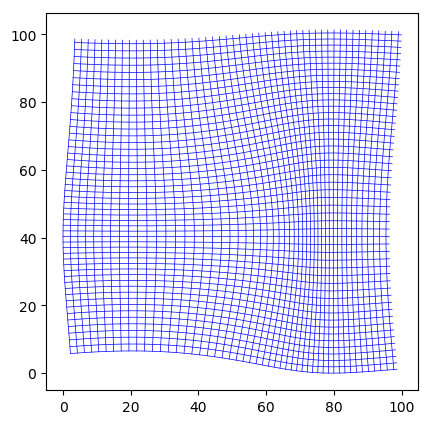
\includegraphics[scale=0.42]{figure/divfree.png}
         \caption{Derived diffeo}
     \end{subfigure}
     \begin{subfigure}[t]{0.45\textwidth}
         \centering
         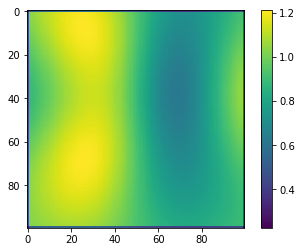
\includegraphics[scale=0.5]{figure/divfree_jacobian.png}
         \caption{Jacobian}
     \end{subfigure}
\end{figure}

What we are trying to do is that, given a set of starting points $\mathbf{p}_i=(x_i,y_i)^T$ and ending points $\mathbf{p}'_i=(x_i+dx_i,y_i+dy_i)^T$ and $\mathbf{d}_i=\mathbf{p}'_i-\mathbf{p}_i=(dx_i,dy_i)^T$, the generated vector field $V$ will satisfy $V(\mathbf{p_i})=\mathbf{d}_i=(dx_i,dy_i)^T$. 

We can generate such vector field in the form of linear combination of feature maps $K_{df}(\cdot,\mathbf{p}_i)$ at $\mathbf{p}_i$:
\begin{equation}
    V(\mathbf{x})=\sum_iK_{df}(\mathbf{x},\mathbf{p}_i)\cdot\mathbf{w}_i,\label{weighted_sum_kernel}
\end{equation}
where $V(\cdot)$ is a RKHS function and $\mathbf{w}_i=(\alpha_i,\beta_i)^T$ is the weight.

\begin{example}
Given only one pair of starting point $\mathbf{p}=(x,y)^T$ and ending point $\mathbf{p}'=(x+dx,y+dy)^T$, the Eq.(\ref{weighted_sum_kernel}) has the form as below
\begin{equation*}
    V(\mathbf{x})=K_{df}(\mathbf{x},\mathbf{p})\cdot\mathbf{w},
\end{equation*}
under the constraint that
\begin{equation*}
    V(\mathbf{p})=K_{df}(\mathbf{p},\mathbf{p})\cdot\mathbf{w}=
    \begin{pmatrix}
    dx\\
    dy
    \end{pmatrix}.
\end{equation*}

Consequently, $\mathbf{w}$ is solved as below
\begin{equation*}
    \begin{pmatrix}
    \frac{1}{\sigma^2} & 0\\
    0 & \frac{1}{\sigma^2}
    \end{pmatrix}\cdot
    \begin{pmatrix}
    \alpha\\
    \beta
    \end{pmatrix}=
    \begin{pmatrix}
    dx\\
    dy
    \end{pmatrix}\rightarrow
    \begin{pmatrix}
    \alpha\\
    \beta
    \end{pmatrix}=
    \begin{pmatrix}
    \sigma^2\cdot dx\\
    \sigma^2\cdot dy
    \end{pmatrix}.
\end{equation*}
\end{example}

\begin{example}
Given $n$ pairs of starting points $\mathbf{p_i}=(x_i,y_i)^T$ and ending points $\mathbf{p_i}'=(x_i+dx_i,y_i+dy_i)^T$, we are to generate the vector field in form of
\begin{equation*}
    V(\mathbf{x})=\sum_i^nK_{df}(\mathbf{x},\mathbf{p}_i)\cdot\mathbf{w}_i
\end{equation*}
under the $n$ constraints that
\begin{align*}
    V(\mathbf{p}_1)=\sum^n_iK_{df}(\mathbf{p}_1&,\mathbf{p}_i)\cdot\mathbf{w}_i=
    \begin{pmatrix}
    dx_1\\
    dy_1
    \end{pmatrix}\\
    &\vdots\\
    V(\mathbf{p}_n)=\sum^n_iK_{df}(\mathbf{p}_n&,\mathbf{p}_i)\cdot\mathbf{w}_i=
    \begin{pmatrix}
    dx_n\\
    dy_n
    \end{pmatrix}
\end{align*}

Incorporating all the constraints above in a matrix form, we can have the equation below
\begin{equation*}
    \begin{pmatrix}
    K_{df}(\mathbf{p}_1,\mathbf{p}_1) & K_{df}(\mathbf{p}_1,\mathbf{p}_2) & \cdots & K_{df}(\mathbf{p}_1,\mathbf{p}_n)\\
    K_{df}(\mathbf{p}_2,\mathbf{p}_1) & K_{df}(\mathbf{p}_2,\mathbf{p}_2) & \cdots & K_{df}(\mathbf{p}_2,\mathbf{p}_n)\\
    \vdots & \vdots & \ddots & \vdots\\
    K_{df}(\mathbf{p}_n,\mathbf{p}_1) & K_{df}(\mathbf{p}_n,\mathbf{p}_2) & \cdots & K_{df}(\mathbf{p}_n,\mathbf{p}_n)\\
    \end{pmatrix}\cdot
    \begin{pmatrix}
    \mathbf{w}_1\\
    \mathbf{w}_2\\
    \vdots\\
    \mathbf{w}_n
    \end{pmatrix}=
    \begin{pmatrix}
    \mathbf{d}_1\\
    \mathbf{d}_2\\
    \vdots\\
    \mathbf{d}_n
    \end{pmatrix}
\end{equation*}

By moving $\mathbb{K}$ to another side, we can solve the $\mathbf{W}$ easily. Since $K_{df}$ is positive-definite matrix, it guarantees that $\mathbb{K}$'s positive-definiteness, which means that $\mathbb{K}$ is always invertable.
\begin{align*}
    &\mathbb{K}\cdot\mathbf{W}=\mathbf{D}\\
    &\mathbf{W}=\mathbb{K}^{-1}\cdot\mathbf{D}
\end{align*}
\end{example}

\section{Appendix}
\subsection{Geodesic Shooting}
Given an initial velocity $v_0\in V$, the geodesic path $t\rightarrow\phi_t\in\mathrm{Diff}^\infty(\Omega)$ under the right-invariant Riemannian metric is uniquely determined by the Euler-Poincare equations(EPDiff)
\begin{equation}
    \frac{\partial v}{\partial t}=-\mathrm{ad}^\dagger_v v=-K\mathrm{ad}^*_vm=-K[(Dv)^Tm+Dmv+m\mathrm{ div } v],
\end{equation}
where $D$ denotes the Jacobian matrix, and the operator $\mathrm{ad}^*$ is the dual of the negative Lie bracket of vector fields,
\begin{equation*}
    \mathrm{ad}_vw=-[v,w]=Dvw-Dwv.
\end{equation*}

By integrating equation (4) forward in time, we generate a time-varying velocity $v_t:[0,1]\rightarrow V$, which itself is subsequently integrated in time by rule $d\phi(x,t)dt=v_t\circ\phi_t(x)$ to arrive at the geodesic path, $\phi(x,t)\in\mathrm{Diff}^s(\Omega)$.

\subsection{PyTorch Tutorial: AUTOGRAD}
\texttt{torch.Tensor} is the central class of the package. If you set its attribute \texttt{.requires\_grad} as \texttt{True}, it starts to track all operations on it. When you finish your computation you can call \texttt{.backward()} and have all the gradients computed automatically. The gradient for this tensor will be accumulated into \texttt{.grad} attribute.

To stop a tensor from tracking history, you can call \texttt{.detach()} to detach it from the computation history, and to prevent future computation from being tracked.

To prevent tracking history (and using memory), you can also wrap the code block in \texttt{with torch.no\_grad():}. This can be particularly helpful when evaluating a model because the model may have trainable parameters with \texttt{requires\_grad=True}, but for which we don’t need the gradients.

There’s one more class which is very important for autograd implementation - a \texttt{Function}.

\texttt{Tensor} and \texttt{Function} are interconnected and build up an acyclic graph, that encodes a complete history of computation. Each tensor has a \texttt{.grad\_fn} attribute that references a Function that has created the Tensor (except for Tensors created by the user - their \texttt{grad\_fn} is \texttt{None}).

If you want to compute the derivatives, you can call \texttt{.backward()} on a \texttt{Tensor}. If Tensor is a scalar (i.e. it holds a one element data), you don’t need to specify any arguments to \texttt{backward()}, however if it has more elements, you need to specify a gradient argument that is a tensor of matching shape. 

Typical pipeline:
\begin{verbatim}
x.requires_grad_()
out = function(x)
out.backward()
gradient = x.grad    
\end{verbatim}

\newpage
\section{Human Connectome}
\subsection{Aim 1: Encoding Connectomes via Riemannian Metrics}
\paragraph{Background}The goal of Aim 1 is to model the individual subject's connectome as a point in the infinite-dimensional space of all Riemannian metrics. In the white matter of the brain, the diffusion of water is restricted perpendicular to the direction of the axons. Thus, the directionality of connections in the brain can be locally inferred as the major eigenvector of the anisotropic diffusion tensors.

However, the inverse diffusion tensor field is not an ideal choice for the Riemannian metric. When using the inverse-tensor metric, geodesics take a shortcut around the high curvature turn of the tract, while geodesics of the conformal Riemannian metric follow the principal eigenvector of the diffusion tensors more faithfully. 

In \cite{hao}, it was assumed that the local Riemannian metric capturing the connectonomics modifies the inverse-tensor estimated from DTI by a spatially varying conformal factor($\alpha$) that causes geodesics to conform more closely to the principal eigenvectors.

\paragraph{Proposed Research: Extending Riemannian Metrics}The method proposed by \cite{hao} has a fundamental limitation that it doesn't generalize to high-angular diffusion-weighted imaging protocol of the human connectome. In the proposed research, we plan to extend the metric estimation problem by allowing the Riemannian metric to vary over the full space of all Riemannian metrics instead of restricting it to a single conformal class.

The completeness of the Riemannian structures is critical to ensure the well-posedness of the regularized inverse problem, which is further discussed in Aim 2.

\subsection{Aim 2: The Geometry of the Manifold of all Riemannian Metrics}
\paragraph{Background} We will describe a mathematical and statistical framework for data analysis of Riemannian metrics and equip the infinite-dimensional space of all Riemannian metrics with an invariant Riemannian metric and base the statistical framework on this infinite-dimensional geometric structure.

We call the Ebin metric natural as it requires no additional background structure and is consequently invariant under the action of the diffeomorphism group, i.e., $G_g(h,k)=G_{\phi^*g}(\phi^*h,\phi^*k)$ for all $\phi\in\mathrm{Diff}(M),g\in\mathrm{Met}(M),h,k\in T_g\mathrm{Met}(M)$.

The invariance of the infinite-dimensional metric under the group of diffeomorphisms is a crucial property, as it guarantees the independence of an initial choice of coordinate system on the brain manifold.

However, the Ebin metric is missing completeness, which is essential for the proposed statistical studies of the human connectome. Bauer et al. introduced a stronger metrics on the space to overcome the obstructions, which can be written as
\begin{equation*}
    G^L(h,k)=\int_M\mathrm{tr}(g^{-1}L_g(h)g^{-1}k)\mathrm{vol}(g)
\end{equation*}
where $L:T\mathrm{Met}(M)\rightarrow T\mathrm{Met}(M)$ is a smooth base-point-preserving bundle isomorphism, such that for every $g\in \mathrm{Met}(M)$, the map $L_g:T_g\mathrm{Met}(M)\rightarrow T_g\mathrm{Met}(M)$ is a pseudo differential operator that is symmetric and positive with respect to the metric $G^E$. 

If the operator field $L$ is invariant under the action of $\mathrm{Diff}(M)$, i.e., $\phi^*(L_gh)=L_{\phi^*g}(\phi^* h)$, then the metric $G^L$ inherits this property and satisfies the same invariance property as the Ebin metric.

\paragraph{Proposed Research: Completeness of Metrics}


\paragraph{Proposed Research: Registering Human Connectomes}
Fundamental to the precise characterization and comparison of the human connectome of an individual subject or a population as a whole is the ability to map or register two different human connectomes. LDDMM can register points, curves and surfaces. This framework has now been extended to densities modeled as volume forms. In this proposal, \underline{we will extend the diffeomorphic mapping framework to the connectome which is modeled as Riemannian metrics.}

With a metric that is invariant, the problem of registering two connectomes fits naturally into the framework of computational anatomy the becomes the following minimization problem:
\begin{equation*}
    E(\phi)=\sigma\mathrm{dist}^2(\mathrm{id},\phi)+\mathrm{dist}^2(g_0,\phi^*g_1)^2
\end{equation*}
The right invariant distance on $\mathrm{Diff}(M)$ is the same as \cite{joshi}.

\paragraph{Proposed Research: Estimating the Average of the Template Connectome of a Population} The existence and uniqueness of the Frechet mean is not guaranteed in general and depend on the completeness and sectional curvature properties of the metric, which are exactly the theoretical goals of previous section. Our statistical framework will be based on the Riemannian structures as described in the first part of Aim 2. We make essential use of the completeness properties of the Riemannian structures to prove well-posedness of the developed statistical framework.

Given a collection of connectomes modeled as points on an abstract Riemannian manifold, we can directly apply the concept of the Frechet mean to define the average connectome.

\paragraph{Proposed Research: Dimensionality Reduction}Principal geodesic analysis (PGA)\cite{pga1,pga2} generalizes PCA to nonlinear manifolds. It describes the geometric variability of manifold data by finding lower dimensional geodesic subspaces that minimize the residual sum-of-squared geodesic distance to the data.

As with the algorithm for estimating the average connectome, the mathematical framework being developed in this proposal will allow us to directly apply the algorithms for performing PGA on collections of connectomes. This will enable us to explicitly visualize and precisely characterize the variability in the architecture of the human connectome of the entire population.

\subsection{Aim 3: Applying the math and statistical framework to DTI}


\newpage
\section{Landmark Matching via Large Deformation Diffeomorphisms\cite{joshi,miller,johnson}}
\subsection{Objective}
Assuming that there is a set of landmarks $\{(x_n,y_n)\}$, where $x_n$ and $y_n$ are  our approach is to construct diffeomorphisms $\phi:\Omega\rightarrow\Omega$, such that
\begin{align}
    \hat{v}(x,t)&=\argmin_vE(v)+D(\phi(\cdot,1))\\ \nonumber
    &=\argmin_v \int^1_0\sum_{n=1}^N\|Lv(x_n,t)\|^2_{L^2}dt+\sum^N_{n=1}[y_n-\phi(x_n,1)]^T\Sigma^{-1}_N[y_n-\phi(x_n,1)],
\end{align}
where
\begin{align*}
    \phi(x,0)&=x\\
    \phi(x,1)&=x+\int^1_0\Dot{\phi}(x,t)dt\\
    \Dot{\phi}(x,t)&=\frac{d\phi(x,t)}{dt}=v(\phi(x,t),t)=v_t\circ\phi_t
\end{align*}

The final time diffeomorphism $\phi(\cdot,1)$ is controlled via the velocity field $v(\cdot,t),t\in[0,1]$. Diffeomorphic landmark transformations are constructed by forcing the velocity fields to minimize quadratic energetic on $\Omega\times[0,1]$, as shown below
\begin{align*}
    E(v)&=\int_0^1\int_\Omega\|Lv(x,t)\|^2_{L^2}dxdt\\
    &=\int_0^1\int_\Omega\sum^{d}_{q=1}|(-\nabla^2+c)v_q(x,t)|^2dxdt
\end{align*} 
since $L$ is in form of $L=I\cdot(-\nabla^2+c)$, where $I$ is the identity matrix, $d$ is the dimension of $v$ and $c$ is a constant.

The squared error distance for landmark matching is given by
\begin{equation*}
    D(\phi(\cdot,1))=\sum^N_{n=1}[y_n-\phi(x_n,1)]^T\Sigma^{-1}_n[y_n-\phi(x_n,1)],
\end{equation*}
where $\Sigma_N$ is the error covariance.

\subsection{Inexact Landmark Matching}
$L$ is a constant coefficient matrix differential operator with $d\times d$ matrix Green's function $G(x,y)$ which is continuous in both $x$ and $y$. Let $K(x,y)=GG^\dagger(x,y)=(2/\sqrt{2\pi c})e^{-\sqrt{c}\|x-y\|}$, where $K$ is a $d\times d$ matrix function. $K$ is the Green's kernel\cite{ref2}. We define the spatial $Nd\times Nd$ covariance matrix $\mathcal{K}(\phi(t))$ as below
\begin{equation*}
    \mathcal{K}(\phi(t))=
    \begin{pmatrix}
    K(\phi(x_1,t),\phi(x_1,t))&\cdots&K(\phi(x_1,t),\phi(x_N,t))\\
    \vdots&\ddots&\vdots\\
    K(\phi(x_N,t),\phi(x_1,t))&\cdots&K(\phi(x_N,t),\phi(x_N,t))
    \end{pmatrix}
\end{equation*}

To express it in a concise way, we have
\begin{equation*}
    \mathcal{K}(\phi(t))_{ij}=K(\phi(x_i,t),\phi(x_j,t))
\end{equation*}

With this, we can rewrite Eq.(1) as
\begin{equation*}
    \hat{v}(x,t)=\sum^N_{i=1}K(\phi(x_i,t),x)\sum^N_{j=1}\mathcal{K}(\phi(t))^{-1}_{ij}\Dot{\hat{\phi}}(x_j,t),
\end{equation*}
where the minimized velocity fields $\Dot{\hat{\phi}}(x_n,t)$ can be expressed as below
\begin{equation}
    \Dot{\hat{\phi}}(x_n,t)=\argmin_{\Dot{\phi}(x_n,\cdot)}\int^1_0\sum^N_{ij=1}\Dot{\phi}(x_i,t)\mathcal{K}(\phi(t))^{-1}_{ij}\Dot{\phi}(x_j,t)dt+\sum^N_{n=1}[y_n-\phi(x_n,1)]^T\Sigma^{-1}_N[y_n-\phi(x_n,1)]
\end{equation}

Assuming velocities are constant within the quantized time intervals, for $t\in[t_{m-1},t_m)$, we have 
\begin{equation*}
    \Dot{\phi}(x_n,t)\approx\frac{\phi(x_n,t_m)-\phi(x_n,t_{m-1})}{\epsilon}
\end{equation*}
where $\epsilon$ is the fixed time step size, such that $t_m=m\epsilon$. 

So the Eq.(2) can have the new form of
\begin{align}
    \hat{\phi}(x_n,t_m)=\argmin& \frac{1}{\epsilon^2}\sum^M_{m=1}\sum^N_{ij=1}[\phi(x_i,t_m)-\phi(x_i,t_{m-1})]^T\left(\int^{t_m}_{t_{m-1}}\mathcal{K}(\phi(t))^{-1}_{ij}dt\right)[\phi(x_j,t_m)-\phi(x_j,t_{m-1})]\\\nonumber
    &+\sum^N_{n=1}[y_n-\phi(x_n,1)]^T\Sigma^{-1}_N[y_n-\phi(x_n,1)]
\end{align}

\subsection{Gradient Algorithm}
The update rule for minimizing Eq.(3) is shown as below
\begin{equation*}
    \phi^{(l+1)}(x_n,t_m)=
    \begin{pmatrix}
    \phi_1^{(l)}(x_n,t_m)\\
    \phi_2^{(l)}(x_n,t_m)\\
    \phi_3^{(l)}(x_n,t_m)\\
    \end{pmatrix}-
    \Delta\times
    \begin{pmatrix}
    \frac{\partial}{\partial\phi_1(x_n,t_m)}P(\phi^{(l)}(1))+\frac{\partial}{\partial\phi_1(x_n,t_m)}D(\phi^{(l)}(1))\\
    \frac{\partial}{\partial\phi_2(x_n,t_m)}P(\phi^{(l)}(1))+\frac{\partial}{\partial\phi_2(x_n,t_m)}D(\phi^{(l)}(1))\\
    \frac{\partial}{\partial\phi_3(x_n,t_m)}P(\phi^{(l)}(1))+\frac{\partial}{\partial\phi_3(x_n,t_m)}D(\phi^{(l)}(1))\\
    \end{pmatrix}
\end{equation*}
where $q=1,2,3$ and $\Delta$ is the step size, rather than Laplacian operator. More explicitly,
\begin{align*}
    \frac{\partial P(\phi(1))}{\partial\phi_q(x_n,t_m)}&=2\sum^N_{j=1}\left(\int^{t_{m+1}}_{t_m}\mathcal{K}(\phi(t))^{-1}_{nj}dt[\phi(x_j,t_m)-\phi(x_j,t_{m+1})]\right)_q\\
    &+2\sum^N_{j=1}\left(\int^{t_m}_{t_{m-1}}\mathcal{K}(\phi(t))^{-1}_{nj}dt[\phi(x_j,t_m)-\phi(x_j,t_{m-1})]\right)_q\\
    &+\sum^N_{j=1}[\phi(x_j,t_{m+1})-\phi(x_j,t_m)]^T\frac{\partial\int^{t_{m+1}}_{t_m}\mathcal{K}(\phi(t))^{-1}_{nj}dt}{\partial\phi_q(x_j,t_m)}[\phi(x_j,t_{m+1})-\phi(x_j,t_m)]\\
    \frac{\partial D(\phi(1))}{\partial\phi_q(x_n,t_m)}&=\delta(t_m-1)(2\Sigma^{-1}_n[y_n-\phi(x_n,1)])_q
\end{align*}
where
\begin{equation*}
    \frac{\partial\int^{t_{m+1}}_{t_m}\mathcal{K}(\phi(t))^{-1}_{nj}dt}{\partial\phi_q(x_j,t_m)}=\int^{t_{m+1}}_{t_m}\left(\mathcal{K}(\phi(t))^{-1}\frac{\partial\mathcal{K}(\phi(t))}{\partial\phi_q(x_j,t_m)}\mathcal{K}(\phi(t))^{-1}\right)_{nj}dt
\end{equation*}
and $\delta(\cdot)$ is the Dirac delta function.

\newpage
\section{Large Deformation Diffeomorphism Metric Matching\cite{beg,tang}}
\subsection{Introduction}
LDDMM is an elegant mathematical formulation shows that the velocity field over time generates diffeomorphisms for large deformation diffeomorphic image registration. This framework introduced a distance metric on the space of diffeomorphisms between images, which gave rise to a variational principle that expresses the optimal image registration as a geodesic flow. The advantages of having a distance metric are
\begin{enumerate}
    \item it formulates a statistical model of the least square problem via minimization of the sum-of-squared residual distance
    \item because this distance between images encodes the information of geometric variability, a number of theoretical methods related to LDDMM.
\end{enumerate}

\subsection{Objective}
A image $I_0$ is deformed by a diffeomorphism $\phi$ as $I_0\circ\phi^{-1}$. Given a source image $I_0$ and a target image $I_1$, we minimize the energy function
\begin{equation*}
    E(v)=\int^1_0\|Lv(t)\|^2_{L^2}dt+\frac{1}{2\sigma^2}\|I_0\circ\phi^{-1}-I_1\|^2_{L^2}
\end{equation*}
which is consisted of a regularization term and a sum-of-squared distance function to estimate diffeomorphic transformation. $\sigma^2$ represents image noise variance. $\|\cdot\|^2_{L^2}$ is equivalent to $|\cdot|^2$.
\begin{figure}[H]
\centering
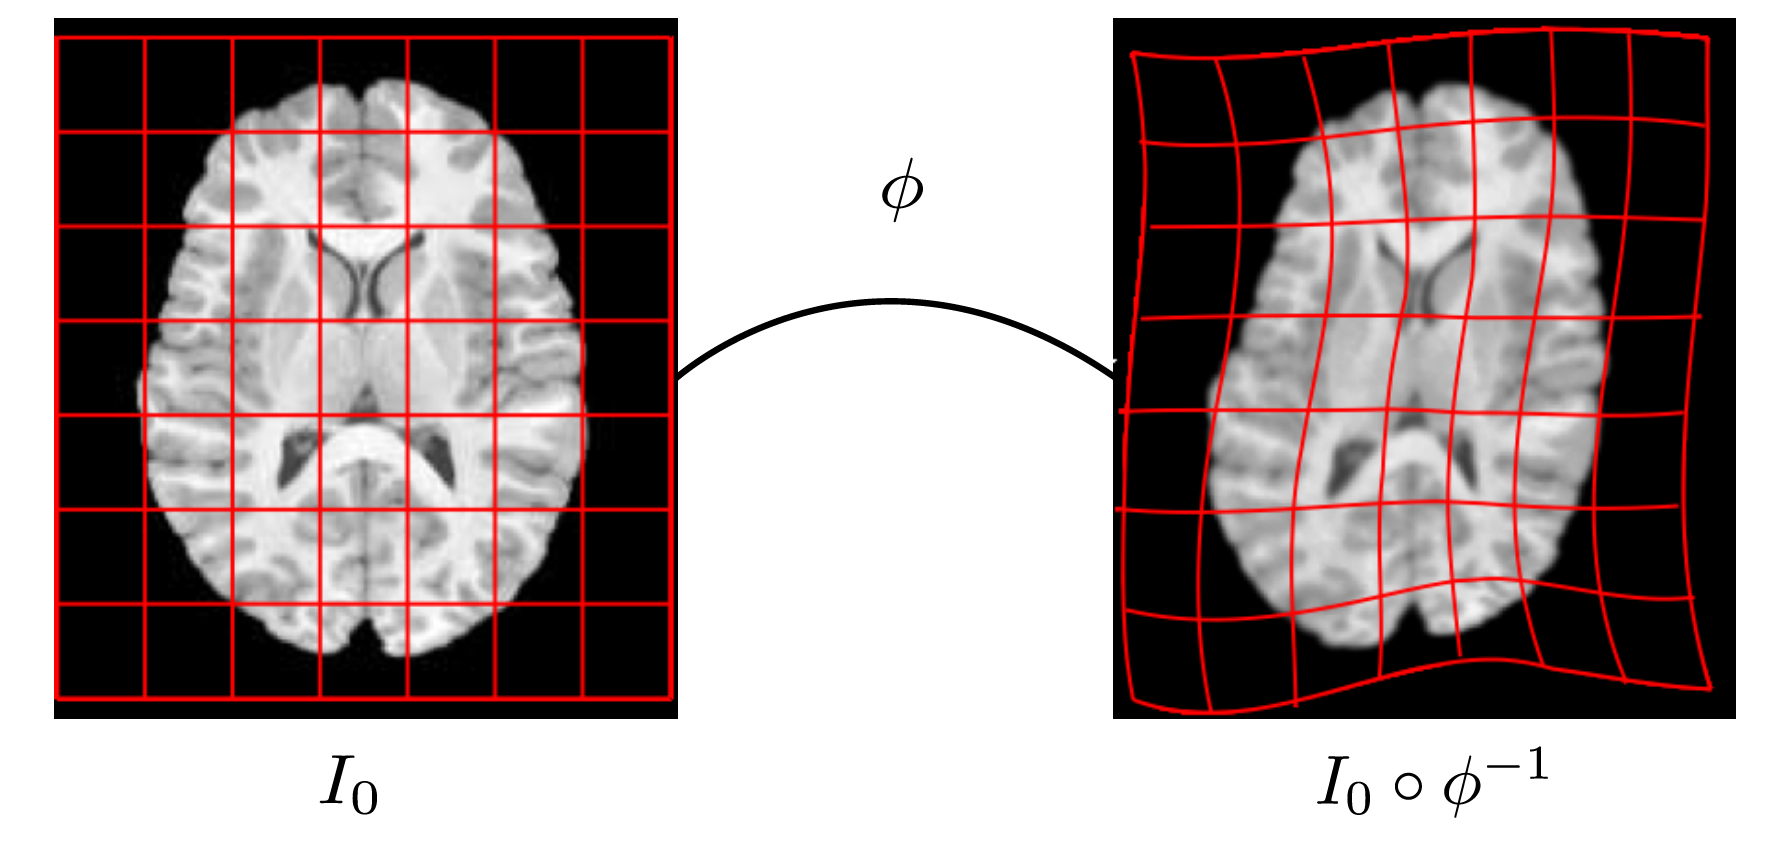
\includegraphics[scale=0.25]{figure/LDDMM.png}
\caption{Deform an axial of a 3D brain MRI image by $\phi$}
\end{figure}

\subsection{Gradient Algorithm}
To ensure that the solution lies in the space of diffeomorphisms, smoothness is achieved by defining the operator $L$ as $L=-\alpha\nabla^2+\gamma I$. In LDDMM, steepest gradient descent approach is used to perform the minimization in energy function and the velocity field at each gradient descent iteration $k$ is updated with
\begin{equation*}
    v^{k+1}(t)=v^k(t)-\varepsilon\nabla_{v^k(t)}E(t),
\end{equation*}
where $\nabla_vE(t)$ as shown below, is the gradient of the energy function
\begin{equation}
    \nabla_vE(t)=2v(t)-K*\left(\frac{1}{\sigma^2}|D\phi_{t,1}^v|\nabla J^0_t(J^0_t-J^1_t)\right)
\end{equation}
where $J^0_t=I_0\circ\phi_{t,0}, J^1_t=I_1\circ\phi_{t,1}, \phi_{s,t}=\phi_t\circ\phi^{-1}_s, K=(L^\dagger L)^{-1}$ and $*$ is the convolution.

Let the velocity $v$ be perturbed by an $\varepsilon$ amount along direction $h$. The Gateaux variation $\partial_hE(v)$ of the energy functional is related to its Frechet derivative $\nabla_vE$ by
\begin{align*}
    \partial_hE(v)&=\lim_{\varepsilon\rightarrow 0}\frac{E(v+\varepsilon h)-E(v)}{\varepsilon}\\
    &=\int^1_0\langle\nabla_vE(t),h(t)\rangledt
\end{align*}

The variation of $E_1(v)=\int^1_0\|v_t\|^2_Vdt=\int^1_0\|Lv_t\|^2_{L^2}dt$ is given by:
\begin{equation*}
    \partial_hE_1(v)=2\int^1_0\langle v_t,h_t\rangle_Vdt.
\end{equation*}

The variation of $E_2(v)=\frac{1}{\sigma^2}\|I_0\circ\phi^v_{1,0}-I_1\|^2_{L^2}$ is
\begin{align*}
    \partial_hE_2(v)&=\frac{2}{\sigma^2}\langle I_0\circ\phi^v_{1,0}-I_1,DI_0\circ\phi^v_{1,0}\cdot\partial_h\phi^v_{1,0}\rangle_{L^2}\\
    &=\frac{2}{\sigma^2}\left< I_0\circ\phi^v_{1,0}-I_1,DI_0\circ\phi^v_{0,1}\cdot\left(-D\phi^v_{1,0}\int^1_0(D\phi^v_{1,t})^{-1}h_t\circ\phi^v_{1,t}dt\right)\right>_{L^2} &&Lemma (1)\\
    &=-\frac{2}{\sigma^2}\int^1_0\langle(I_0\circ\phi^v_{1,0}-I_1,D(I_0\circ\phi^v_{1,0})\cdot(D\phi^v_{1,t})^{-1}\cdot h_t\circ\phi^v_{1,t}\rangle_{L^2}dt
\end{align*}
\begin{lemma}
The variation of mapping $\phi^v_{s,t}$ when $v\in L^2$ is perturbed along $h\in L^2$ is given by
\begin{align*}
    \partial_h\phi^v_{s,t}&=\lim_{\varepsilon\rightarrow0}\frac{\phi^{v+\varepsilon h}_{s,t}-\phi^v_{s,t}}{\varepsilon}\\
    &=D\phi^v_{s,t}\int^t_s(D\phi^v_{s,t})^{-1}h_u\circ\phi^v_{s,u}du
\end{align*}
\end{lemma}
\begin{align*}
    \partial_hE_2(v)&=-\frac{2}{\sigma^2}\int^1_0\langle|D\phi^v_{t,1}|(I_0\circ\phi^v_{t,0}-I_1\circ\phi^v_{t,1}),D(I_0\circ\phi^v_{t,0})h_t\rangle_{L^2}dt\\
    &=-\frac{2}{\sigma^2}\int^1_0\langle|D\phi^v_{t,1}|(J^0_t-j^1_t)\nabla J^0_t,h_t\rangle_{L^2}dt\\
    &=-\int^1_0\left< K\left(\frac{2}{\sigma^2}|D\phi^v_{t,1}|(J^0_t-J^1_t)\nabla J^0_t\right),h_t\right>_Vdt
\end{align*}
where the subscript $V$ indicates the gradient is in the space $V$.

Collecting terms, the gradient of the energy functional is thus
\begin{equation*}
    \nabla_vE_t=2v_t-K\left(\frac{2}{\sigma^2}|D\phi^v_{t,1}|\nabla J^0_t(J^0_t-J^1_t)\right )
\end{equation*}
The optimizing velocity field satisfies the Euler-Lagrange equation
\begin{equation*}
    \partial_hE(\hat{v})=\int^1_0\left<2\hat{v}_t-K\cdot\left(\frac{2}{\sigma^2}|D\phi^\hat{v}_{t,1}|\nabla|J^0_t(J^0_t-J^1_t)\right),t_t\right>_Vdt=0,
\end{equation*}
since $h$ is arbitrary in $L^2([0,1],V)$ we get Eq.(4).

In the numerical implementation of LDDMM, the time parameter $t$ of the flow is discretized with a fixed total number of time steps $T$, where $T=10$ is selected as the default descent to terminate with a higher final mismatch error $\|I_0\circ\phi^{-1}-I_1\|^2_{L^2}$ between the registered atlas image and the target image. 

The convolution operation in Eq.(4) is calculated in Fourier domain. The operator $K$ acts as a low pass filter at each iteration of gradient descent and the parameters $\alpha$ and $\gamma$ controls the amount of smoothing and the elasticity of the deformation. Selection of these parameters depends on the size of the deformation necessary to register the features of the atlas image to the features of the target image

\begin{thebibliography}{99} 
\bibitem{joshi}Joshi, S.C. and Miller, M.I., 2000. \textit{Landmark matching via large deformation diffeomorphisms}. IEEE transactions on image processing, 9(8), pp.1357-1370.
\bibitem{miller}Miller, M.I., Trouvé, A. and Younes, L., 2002. \textit{On the metrics and Euler-Lagrange equations of computational anatomy}. Annual review of biomedical engineering, 4(1), pp.375-405.
\bibitem{johnson}Johnson, H.J. and Christensen, G.E., 2001, June. \textit{Landmark and intensity-based, consistent thin-plate spline image registration}. In Biennial International Conference on Information Processing in Medical Imaging (pp. 329-343). Springer, Berlin, Heidelberg.
\bibitem{tang}Ceritoglu, C., Tang, X., Chow, M., Hadjiabadi, D., Shah, D., Brown, T., Burhanullah, M.H., Trinh, H., Hsu, J., Ament, K.A. and Crocetti, D., 2013. \textit{Computational analysis of LDDMM for brain mapping. Frontiers in neuroscience}, 7, p.151.
\bibitem{beg}Beg, M.F., Miller, M.I., Trouvé, A. and Younes, L., 2005. \textit{Computing large deformation metric mappings via geodesic flows of diffeomorphisms}. International journal of computer vision, 61(2), pp.139-157.
\bibitem{pga1}Fletcher, P.T., Lu, C. and Joshi, S., 2003, June. \textit{Statistics of shape via principal geodesic analysis on Lie groups}. In 2003 IEEE Computer Society Conference on Computer Vision and Pattern Recognition, 2003. Proceedings. (Vol. 1, pp. I-I). IEEE.
\bibitem{pga2}Fletcher, P.T., Lu, C., Pizer, S.M. and Joshi, S., 2004. \textit{Principal geodesic analysis for the study of nonlinear statistics of shape}. IEEE transactions on medical imaging, 23(8), pp.995-1005.
\bibitem{hao}Hao, X., Zygmunt, K., Whitaker, R.T. and Fletcher, P.T., 2014. \textit{Improved segmentation of white matter tracts with adaptive Riemannian metrics}. Medical image analysis, 18(1), pp.161-175.
\bibitem{jacobi}Logarithm of a matrix: A Lie group theory perspective. Wikipedia. \url{https://en.wikipedia.org/wiki/Logarithm_of_a_matrix}
\bibitem{hinkle}Hinkle, J. and Joshi, S., 2013, June. \textit{Idiff: irrotational diffeomorphisms for computational anatomy}. In International Conference on Information Processing in Medical Imaging (pp. 754-765). Springer, Berlin, Heidelberg.
\bibitem{khesin}Khesin, B., Lenells, J., Misiolek, G. and Preston, S.C., 2011. \textit{Geometry of diffeomorphism groups, complete integrability and optimal transport}. arXiv preprint arXiv:1105.0643.
\bibitem{macedo}Macêdo, I. and Castro, R., 2010. Learning divergence-free and curl-free vector fields with matrix-valued kernels. IMPA.
\end{thebibliography}
\end{document}
